%% Copernicus Publications Manuscript Preparation Template for LaTeX Submissions
%% ---------------------------------
%% This template should be used for copernicus.cls
%% The class file and some style files are bundled in the Copernicus Latex Package, which can be downloaded from the different journal webpages.
%% For further assistance please contact Copernicus Publications at: production@copernicus.org
%% https://publications.copernicus.org/for_authors/manuscript_preparation.html


%% Please use the following documentclass and journal abbreviations for preprints and final revised papers.

%% 2-column papers and preprints
\documentclass[journal abbreviation, manuscript]{copernicus}


%% Journal abbreviations (please use the same for preprints and final revised papers)


% Advances in Geosciences (adgeo)
% Advances in Radio Science (ars)
% Advances in Science and Research (asr)
% Advances in Statistical Climatology, Meteorology and Oceanography (ascmo)
% Aerosol Research (ar)
% Annales Geophysicae (angeo)
% Archives Animal Breeding (aab)
% Atmospheric Chemistry and Physics (acp)
% Atmospheric Measurement Techniques (amt)
% Biogeosciences (bg)
% Climate of the Past (cp)
% DEUQUA Special Publications (deuquasp)
% Earth Surface Dynamics (esurf)
% Earth System Dynamics (esd)
% Earth System Science Data (essd)
% E&G Quaternary Science Journal (egqsj)
% EGUsphere (egusphere) | This is only for EGUsphere preprints submitted without relation to an EGU journal.
% European Journal of Mineralogy (ejm)
% Fossil Record (fr)
% Geochronology (gchron)
% Geographica Helvetica (gh)
% Geoscience Communication (gc)
% Geoscientific Instrumentation, Methods and Data Systems (gi)
% Geoscientific Model Development (gmd)
% History of Geo- and Space Sciences (hgss)
% Hydrology and Earth System Sciences (hess)
% Journal of Bone and Joint Infection (jbji)
% Journal of Micropalaeontology (jm)
% Journal of Sensors and Sensor Systems (jsss)
% Magnetic Resonance (mr)
% Mechanical Sciences (ms)
% Natural Hazards and Earth System Sciences (nhess)
% Nonlinear Processes in Geophysics (npg)
% Ocean Science (os)
% Polarforschung - Journal of the German Society for Polar Research (polf)
% Primate Biology (pb)
% Proceedings of the International Association of Hydrological Sciences (piahs)
% Safety of Nuclear Waste Disposal (sand)
% Scientific Drilling (sd)
% SOIL (soil)
% Solid Earth (se)
% State of the Planet (sp)
% The Cryosphere (tc)
% Weather and Climate Dynamics (wcd)
% Web Ecology (we)
% Wind Energy Science (wes)

%% \usepackage commands included in the copernicus.cls:
%\usepackage[german, english]{babel}
%\usepackage{tabularx}
%\usepackage{cancel}
%\usepackage{multirow}
%\usepackage{supertabular}
\usepackage{algorithmic}
\usepackage{algorithm}
%\usepackage{amsthm}
%\usepackage{float}
%\usepackage{subfig}
%\usepackage{rotating}
%\usepackage{geometry}
%\usepackage{booktabs}
%\usepackage{siunitx}
\usepackage{graphicx}
\usepackage{rotating}
\usepackage{longtable}
\usepackage{booktabs}
\usepackage{subcaption}
\usepackage{cleveref}

\usepackage[version=4]{mhchem}
\begin{document}

\title{NN-TOC v1: GLOBAL PREDICTION OF TOTAL ORGANIC CARBON IN MARINE SEDIMENTS USING DEEP NEURAL NETWORKS}

\Author[1,2]{Naveenkumar}{Parameswaran}
\Author[1]{Everardo}{Gonz\'{a}lez}
\Author[3]{Ewa}{Burwicz-Galerne}
\Author[2]{Malte}{Braack}
\Author[1]{Klaus}{Wallmann}



\affil[1]{GEOMAR Helmholtz Centre for Ocean Research Kiel, Kiel, Germany}
\affil[2]{Department of Mathematics, Kiel University, Kiel, Germany}
\affil[3]{MARUM - Center for Marine Environmental Sciences, University of Bremen, Bremen, Germany}


%% If authors contributed equally, please mark the respective author names with an asterisk, e.g. "\Author[2,*]{Anton}{Smith}" and "\Author[3,*]{Bradley}{Miller}" and add a further affiliation: "\affil[*]{These authors contributed equally to this work.}".developed new methods


\correspondence{Naveenkumar Parameswaran (nparameswaran@geomar.de)}

\runningtitle{TEXT}

\runningauthor{TEXT}





\received{}
\pubdiscuss{} %% only important for two-stage journals
\revised{}
\accepted{}
\published{}

%% These dates will be inserted by Copernicus Publications during the typesetting process.


\firstpage{1}

\maketitle



\begin{abstract}
Spatial predictions of total organic carbon (TOC) concentrations and stocks are crucial for understanding marine sediments’ role as a significant carbon sink in the global carbon cycle. In this study, we present a geospatial prediction of global TOC concentrations and stocks on a 5 x 5 arc minute grid, using a novel neural network approach. We also provide and apply a new compilation of over 21,000 global TOC measurements and a new set of predictors including features such as seafloor lithologies, benthic oxygen fluxes, and chlorophyll-a satellite data. Moreover, we compare different machine learning models based on their performance metrics and predictions and assess their strengths and limitations. For the dataset used, we find that the performance metrics of the models are comparable and the neural network approach outperforms on unseen data compared to methods such as k Nearest Neighbors and random forests, which tend to overfit to the training data. We provide estimates of mean TOC concentrations and stocks in both continental shelves and deep-sea settings across various marine regions and oceans. Our model suggests that the upper 10 $cm$ of oceanic sediments harbor approximately 156 $Pg$ of TOC stock and has a mean TOC concentration of 0.61\%. Furthermore, we introduce a standardized methodology for quantifying predictive uncertainty using Monte Carlo dropout. The method was applied to our neural network model and underlying features to generate a map of information gain, that measures the expected increase in model knowledge, achieved through additional sampling at specific locations which is pivotal for sampling strategy planning.
\end{abstract}




\introduction  
\label{sec:Introduction}



Burial of particulate organic carbon in marine sediments removes carbon dioxide (\ce{CO2}) from the atmosphere and generates molecular oxygen (\ce{O2}) that accumulates in the atmosphere \citep{Berner1982, HEDGES199581}. It is a key process in the global carbon cycle that largely controls the atmospheric partial pressures of \ce{O2} and \ce{CO2} on geological timescales \citep{Berner1982, bernerbook2004}. The mechanisms controlling concentrations, standing stocks, degradation and accumulation rates of organic carbon at the seabed are, however, complex and remain a topic of active research \citep{ARNDT201353, burdige2007, HEDGES199581, larowe2020a, Bradley2022}.  Furthermore, present estimates on the spatial distribution of sedimentary carbon concentrations and stocks across the global ocean, including shelf regions, are limited due to sparse data and the large spatial variability observed in shelf deposits \citep{atwood2020, diesing2021, LeeTOCkNN, legge2020, SEITER20042001}. An improved map of global organic carbon concentrations and stocks in marine surface sediments, including the continental shelf, could, hence, help to better understand processes governing the turnover and accumulation of organic carbon at the seabed.


%Shelf and deep-sea regions are separate environments. Surface sediments deposited on the continental shelf are mostly composed of clay, silt, and sand delivered by rivers and continental erosion, while pelagic sediments deposited at the deep-sea floor contain large amounts of biogenic material (carbonate, biogenic opal) produced by marine plankton \citep{bernerAndBerner2012}. Moreover, shelf deposits are frequently eroded, reworked and redistributed by bottom currents and intensively mixed and irrigated by benthic biota \citep{ALLER1998143, boudreau1997diagenetic, song2022global}. Shelf sediments are also affected by human activities such as bottom-trawling and dredging that erode and disperse large sediment volumes \citep{Sala2021, Oberle2016}. Organic carbon within shelf and deep-sea deposits constitutes only a minor fraction of the sediment mass. It is composed of both reactive and inert organic matter where the reactive fraction is subject to fast biological degradation processes \citep{Hiddink2023}. Degradation rates increase with temperature and oxygen exposure \citep{ARNDT201353, HEDGoveresES199581}. Global warming and resuspension of anoxic shelf sediments in oxygen-bearing bottom waters by e.g. bottom-trawling, therefore, enhance organic carbon degradation and induce significant \ce{CO2} emissions at the seabed that may contribute to global climate change \citep{Hiddink2023, Sala2021}. An improved understanding of carbon stocks in surface sediments and their spatial distribution is, hence, also needed to better constrain present and future \ce{CO2} fluxes at the shelf seabed \citep{atwood2020}.


Sedimentary organic carbon concentrations are typically reported as total organic carbon (TOC in weight percent), which includes particulate organic carbon bound to sediment grains and a minor contribution by organic carbon dissolved in sediment porewater \citep{HEDGES199581}. TOC varies between different geological environments \citep{Emerson1988}. Fine-grained shelf and delta sediments deposited close to river mouths typically contain 0.5 – 1.0\% TOC at 0 – 10 $cm$ sediment depth \citep{Berner1982}. A major fraction of TOC deposited in these environments (up to 67\%) is not formed by marine plankton but produced by land plants \citep{Burdige2005}. Shelf regions where neritic carbonates are formed by corals and other organisms at the seabed contain about 1\% TOC \citep{Berner1982}. However, large parts of the continent shelf (about 50 - 70\%) do not receive sediment inputs and are covered by relict sands \citep{emery1968relict, Hall2002} that contain only minor amounts of TOC (about 0.1\%). Typical deep-sea sediments, that are not associated with high productivity regions, contain about 0.2 – 0.4\% TOC \citep{Baturin2007, Berner1982, LeeTOCkNN, SEITER20042001}. In oceanic upwelling regions with high productivity, large amounts of TOC are rapidly deposited at the seabed such that sedimentary TOC concentrations are usually larger than 1\% and may reach up to 10\% \citep{Berner1982, LeeTOCkNN, SEITER20042001}. Elevated TOC values are also reported for surface sediments deposited in the Arctic Ocean (1.0\%) and the deep basins of the Black Sea (2.0\%) \citep{Berner1982, LeeTOCkNN, SEITER20042001}. Considering these observations, the global mean TOC concentration in both shelf and deep-sea sediments seems to be close to 0.5 to 1.0\%.


The inventory or standing stock of TOC in surface sediments (in mass of carbon per seafloor area) is calculated by multiplying TOC concentrations with the dry bulk density of sediments and the thickness of the considered surface layer. Different methods have been applied to derive the standing stock of TOC at regional and global scales. An early estimate based on limited data and expert knowledge concluded that the global TOC stock is 146 $Pg$ TOC for a 30 $cm$ thick surface layer \citep{Emerson1988}. The first estimate of the global TOC inventory derived by a machine-learning approach (k-Nearest Neighbors (kNNs)) using an extended database (5,623 data points) yielded a global inventory of 87 $\pm$ 43 $Pg$ TOC in the top 5 $cm$ layer \citep{LeeTOCkNN}. In subsequent publications with an extended database (11,574 sediment cores) and a more advanced machine-learning approach (random forest model), the global inventory was estimated as 2322 $Pg$ TOC for the top 1 $m$ of the sediment column \citep{atwood2020}. This inventory exceeds the global TOC inventory in terrestrial soils and suggests that TOC in marine surface sediments is the largest TOC pool at the surface of the Earth \citep{atwood2020}. Another estimate of the global TOC inventory was derived by reactive transport modeling of sedimentary processes employing a range of global datasets \citep{larowe2020b}. This model yields a global inventory of 170 $Pg$ TOC for the top 10 $cm$ affected by biological mixing processes.% in a baseline scenario, which represents various depositional environments, while the model gives 170 $Pg$ and 111 $Pg$ with parameters chosen for low reactivity scenario for high reactivity scenarios. 


Since about 70\% of the Earth's surface is covered by oceans, and sampling sediments at the seafloor is costly, data coverage will always be sparse. Therefore, advanced methods are required to derive spatial information on sediment properties from a limited number of point measurements. Machine learning approaches, which have rapidly advanced in recent years, are the most promising approach to tackle this challenge. So far, k-nearest neighbors and random forest models have been applied to derive global maps of sediment porosity \citep{Martin2005Porosity}, TOC concentration \citep{LeeTOCkNN}, TOC inventory \citep{atwood2020}, sedimentation rate \citep{restrepo2, Restreppo2020}, and regional estimates of TOC accumulation rates \citep{diesing2021}. However, machine-learning techniques have their own challenges and limitations. Overfitting issues are often encountered, and a standardized approach for estimating predictive uncertainty has not yet been established \citep{LeeTOCkNN}.



Given these challenges, this paper aims to derive more robust maps of TOC concentrations and inventories for the global ocean. These maps, including the continental shelf, are based on a new larger TOC measurement database and an extended collection of predictors to improve the accuracy of predictions for highly heterogeneous and undersampled geological settings. We compiled an enlarged database of TOC concentrations in surface sediments with 21,125 entries and applied a deep neural network (DNN) as a more advanced machine-learning approach that considers the non-linear relationships between TOC and other geological features. The global ocean was divided into two different domains (shelf and deep-sea), and the network was trained separately for each of these domains. Moreover, we introduced a standardized methodology called Monte Carlo Dropout to quantify predictive uncertainties in the DNN model and derive information gain to guide future sampling efforts.



\section{Materials}
\subsection{Features}
\label{sec:features}
An extensive repository of features from both the sea surface and the seafloor at a 5 x 5 arc minute grid resolution has been compiled using previously reported feature lists \citep{LeeTOCkNN, restrepo2, HartDavis2021EOT20} that include a range of oceanographic, geological, geographic, biological, and biogeochemical parameters. It is worth noting that oceanographic features are updated very often from newer models and measurements, and some of the features used here might be outdated. Features deemed irrelevant to TOC distributions (e.g. crustal and mantle properties; distance to plate boundary, continental ridges, trenches) were excluded. Additional features that may influence TOC distributions were added to improve TOC predictions. These include total oxygen uptake (respiration rates) at the seabed  \citep{TOU_JORGENSEN2022}, sediment lithology \citep{garlan2018}, tidal velocities \citep{HartDavis2021EOT20}, and chlorophyll-a concentrations at the sea surface \citep{nasaaqua}.


99 raw feature grids are compiled for a comprehensive representation of the marine environment, providing the necessary input for the neural network analysis in this study to predict TOC concentrations in marine sediments. Most of these features are easily measurable from the sea surface by e.g. satellite observations, making them a reliable dataset compared to the less accessible properties of the seafloor. Some of the seafloor feature grids used in this work were previously generated from raw data using machine-learning methods (e. g. porosity grid provided by \cite{Martin2005Porosity}). Others were reprocessed in this work to achieve global coverage at a resolution of 5 x 5 arc minutes (e.g. sediment lithology \citep{garlan2018}).

Neighborhood information was incorporated for a subset of the features. Specifically, 40 of the initial 99 features were spatially averaged using a 50 km radius \citep{LeeTOCkNN}. Spatial averaging was applied when TOC concentrations are assumed to be affected not only by the local feature value but also by feature values  in the surrounding area.  This approach was used for selected physical (e.g., current velocity), chemical (e.g., dissolved compounds), and biological parameters (e.g., biofauna abundance). 

Overall, a total of 139 features including 99 original features and 40 additional spatially averaged features are used in the model. The complete feature list is presented in Appendix \ref{appendix:featurelist}.



\subsection{TOC Data}
\label{subsec: labels}
The dataset for TOC concentrations (in weight percent) utilized in this study has been compiled from multiple sources. It includes global data sets \citep{SEITER20042001, romankevich2009organic, mosaic, mosaicv2} and regional data sets for the northern Gulf of Mexico \citep{beazley2003significance} and the North Sea (personal communication, W. Zhang, HEREON). Each label represents a known measurement (TOC concentration) and is paired with the nearest grid point on the 139-feature grids via L2 distance computation, resulting in the association of a feature vector with each label. For those stations where TOC is reported as function of sediment depth, we calculated the mean TOC concentration for the top 10 $cm$ and used this mean as model label. For many stations, values are only reported for the top 1-2 $cm$ (around 19,000 measurements). We included these stations in our model since they contain valuable information but acknowledge that they may be somewhat higher than those integrated over the top 10 $cm$ since TOC concentrations tend to decrease with sediment depth due to ongoing TOC degradation. However, most sediments deposited on the continental shelf and in high-productivity regions of the open ocean are affected by intense biogenic and physical mixing processes \citep{boudreau1997diagenetic} such that the down-core TOC decrease is usually small within the mixed surface layer (0 – 10 $cm$ sediment depth) The labeled data is preprocessed to enhance the reliability and robustness of the dataset for subsequent model development and validation. We first searched for duplicates in our combined data base that may arise when the same data are reported in multiple data bases. They were removed from the combined data base when longitudes, latitudes and TOC concentrations were identical. Moreover, coastal regions often exhibit clustered measurements, potentially resulting in shared feature vectors, as all the measurements lie in the same feature grid cell. To mitigate this, a variance assessment is conducted. Labels, that share the same feature vectors, exhibiting high variance (the standard deviation of these labels is higher than 20\% of the maximum of these labels) are excluded, while those with low variance are averaged, and the shared feature vector is assigned. Also, some data points situated in close proximity to land were not adequately captured by the 5 x 5 arc minute grid. To address this, reasonable values are assigned by interpolating from the nearest points, ensuring the overall quality of the dataset. Our database includes a total of 110,149 data points that have been consolidated as discussed above such that the final TOC database employed in the model is composed of 21,125 entries
 (Figure \ref{fig:toclabels}). Both the datasets for labels and features can be downloaded at https://doi.org/10.5281/zenodo.11186224.

\begin{figure}[!htb]
    \includegraphics[width=12cm]{figures/f01.png}
    \caption{Quantitative TOC measurements (i.e., labels) acquired from various sources \citep{SEITER20042001, romankevich2009organic, mosaic, beazley2003significance, mosaicv2}. Notably, data point clusters are observed in close proximity to coastal regions\footnote{The color maps used for the figures in this paper are from \cite{fabiocramericolormap} and \cite{cmoceancolormap}.}.}
    \label{fig:toclabels}
\end{figure}




\section{Methods}
\label{sec:methods}

The primary objective of this study is to build a supervised prediction model that uses feature grid maps as inputs to predict TOC concentrations as outputs. Additionally, we aim to quantify prediction uncertainties using Monte Carlo dropout and information theory techniques. The supervised model is trained using the set of labels (TOC data) and their corresponding feature vectors. Due to the non-linearity in the relationships between data and features, we choose deep learning models, which are good at understanding such patterns. Deep Neural Networks (DNNs) transform data non-linearly with non-linear activation functions such as ReLU (Rectified Linear Unit), a piecewise linear function that outputs 0 for negative inputs and the input itself for positive inputs, introducing non-linearity in the DNN. Therefore, even after one layer, multicollinearity in the data is eliminated. In our case of a deep neural network, the final output is controlled by  numerous combinations of ReLU functions involving higher order interactions of original features  \citep{devaux1994}.


\subsection{Deep learning model}
Deep Neural Networks have achieved state of the art results on a variety of tasks in ocean observation, prediction, and forecasting of ocean phenomena \citep{reviewAIinMarineScience}. DNN architectures, that are intrinsically non-parametric and non linear, are less susceptible to the curse of dimensionality. They capture complex relationships between data and features at different levels of abstraction through their hierarchical nature which makes them well-suited to resolve highly complex geoscientific problems \citep{LeCun2015}. 

Here, we use a multi-layer perceptron (MLP), feed forward DNN to predict global TOC in sediments and introduce a new approach to map uncertainty in predictions that serves as a quantifiable measure of information gain from sampling. To further improve our predictions,  the global ocean was separated into a continental shelf and deep-sea region using the 200$m$ water depth horizon as a boundary.  Two separate models were trained for these regions (shelf: 0 - 200 m, deep-sea: > 200$m$)  to consider the different processes that drive sedimentation and control TOC values in the deep-sea and shelf environment. The same set of features is used for both regions, but the interplay of these features differs between the contrasting environments. The weights and the biases in the DNN is initialized using the technique proposed by \cite{he2015delving}. Batch normalization (which normalizes the inputs of each layer for faster and more stable training) and dropout (which assigns a probability of being deactivated to each node during training and thus prevents overfitting) are applied to each layer for regularization. ReLU is used as the activation function. 



The Monte Carlo Dropout method is implemented here to estimate uncertainty in the DNN model, leveraging dropout layers as approximate Bayesian inference \citep{MCDropout}. It gives us an ensemble of predictions from different subsets of neurons in the same DNN model. Kullback Leibler (KL) divergence is used to map information gain from the quantified predictive uncertainty. In the field of information theory, KL divergence represents the information gain and is defined as the difference of the cross entropy between the observation and the prediction of an event, and the entropy in the observation of the event \citep{kullbackleibler1951}. In our context, the predicted distribution arises from Monte Carlo dropout prediction ensemble, while the reconstructed observed distribution is modeled with a normal distribution with the predicted value as a mean and the standard deviation of 0.05 TOC\%, arising from both technical handling and the precision of the weighing tool \citep{pape2020}.

Uncertainty and information gain are inherently associated in as far as there cannot be high information gain without high uncertainty, however, information gain also depends on the observation probability distribution and is constrained by it. In other words, information gain measures the expected increase in model knowledge achieved through field sampling at a specific location. This concept provides a strategic guide for determining optimal sampling strategies: taking samples in regions with the highest information gain values is the most efficient way to refine our model’s representation of the real world. The mathematical formulation of entropy, cross entropy, and information gain is detailed in Appendix \ref{appendix:informationgain}.

%


\section{Results and Discussions}
Understanding the global distribution of TOC concentrations and stocks is crucial for advancing our knowledge of the carbon cycle and sedimentary environments worldwide. Before delving into the prediction maps from the DNN, we first compare the performance of three methods: DNNs, kNNs, and random forests. Separate models are run for deep-sea and continental shelf regions, and the outcomes are summarized in Table \ref{tab:kNNRF}. For kNN, 5 neighbors were utilized for continental shelves, and 4 for the deep-sea, based on a sensitivity analysis with respect to model performance. Random forests employed 100 estimators for both marine regions. The DNN consists of 10 layers with 128 nodes each. The choice of hyperparameters in the models are discussed in Appendix \ref{appendix:kNNRF}. This comparison sets the groundwork for a detailed exploration of DNN results. All the methods were run with the same train/test splits of the dataset and the random split is seeded to make the methods reproducible. 

The results of this model comparison show that random forest and kNN algorithms exhibit higher correlation coefficients and superior overall performance on the training dataset than the DNN. However, the DNN outperforms the other two algorithms in the test data performance (Table \ref{tab:kNNRF}), for the dataset used. This discrepancy suggests a potential overfitting issue, where the kNN and random forest models may have become specialized in learning the training data. The emphasis on generalization capabilities is crucial in our context due to data scarcity in many regions, making predictions in unexplored  areas a priority. The correlation plot between measured and predicted data shows similar errors for the training and test data sets which confirms that the DNN-model largely avoids overfitting (Figure \ref{fig:correlationPlot}). The observed underestimation of TOC concentrations at higher values is likely due to the distribution of the ground truth dataset, which is predominantly composed of low TOC concentrations (<1\%). Training an NN model on such an imbalanced dataset often results in a model that is biased toward predicting lower values, effectively "erring on the side of caution". 
Several approaches could be employed to address this issue, such as weighting the gradient descent steps based on concentration values, applying a logarithmic transformation to the TOC scale, or balancing the dataset by withholding low-value labels. However, each of these methods is likely to introduce trade-offs, potentially reducing accuracy in other areas.Ultimately, the most effective way to improve the model's performance in predicting higher TOC concentrations is to obtain additional TOC samples within this higher range.

The prediction map of DNN is presented in figure \ref{fig:tocPercent} while maps generated by kNN and random forests are provided in Appendix \ref{appendix:kNNRF} (Figure \ref{fig:tocPercent_kNN}, \ref{fig:tocPercent_RF}). Both the kNN and random forests showed artifacts particularly in the equatorial Pacific and Atlantic oceans, similar to the map published by \cite{LeeTOCkNN}. As stated by \cite{LeeTOCkNN}, there is no standard means of quantifying uncertainty in kNN. In random forests, the variance or standard deviation of all the sub-output values to measure the regression uncertainty is considered as an uncertainty quantification method, but it is difficult to provide the uncertainty for an individual base learner \citep{Mentch2016}. Estimating the confidence of the predictions should be an important factor in deciding which model to use. On the other hand, uncertainty quantification in DNN is an active field of research and has standardized methods. Nonetheless, kNNs and random forests are useful learning algorithms when computational resources are constrained and requires an out-of-the-box solution.

We also tested a DNN model where the global ocean was not separated into shelf and deep-ocean regions but treated as one entity. The resulting TOC map shows spurious features in the Pacific Ocean (Appendix \ref{appendix:entireModel}), similar to those that occur in previous predictions. This additional model shows that the separation of the ocean into shelf and deep-sea regions improves the model results. 


\begin{table}[h]
  \centering
  \begin{tabular}{|l|c|c|c|c|c|c|}
    \hline
    \textbf{Method} & \multicolumn{3}{c|}{\textbf{Train data}} & \multicolumn{3}{c|}{\textbf{Test data (15\% of all data)}} \\
    \hline
           & \textbf{Pearson CC} & \textbf{R-squared} & \textbf{MSE} & \textbf{Pearson CC} & \textbf{R-squared} & \textbf{MSE}\\
    \hline
    \textbf{kNN} & 0.921& 0.45& 0.517& 0.852& 0.719& 0.541\\
    \hline
    \textbf{Random forests} & \textbf{0.986} & \textbf{ 0.966} & \textbf{0.239} &  0.867& 0.745& \textbf{0.499}\\
    \hline
    \textbf{DNN} & 0.928 & 0.844& 0.492& \textbf{0.888}&\textbf{ 0.737}& 0.537\\
    \hline
  \end{tabular}
    \caption{Comparison of machine learning methods based on performance metrics: Pearson correlation coefficient (Pearson CC), coefficient of determination (R-Squared), and mean squared error for predicted values vs observed labels for the training and testing data. The train:test data ratio is 85:15.}
  \label{tab:kNNRF}
\end{table}




\begin{figure}
    \centering
    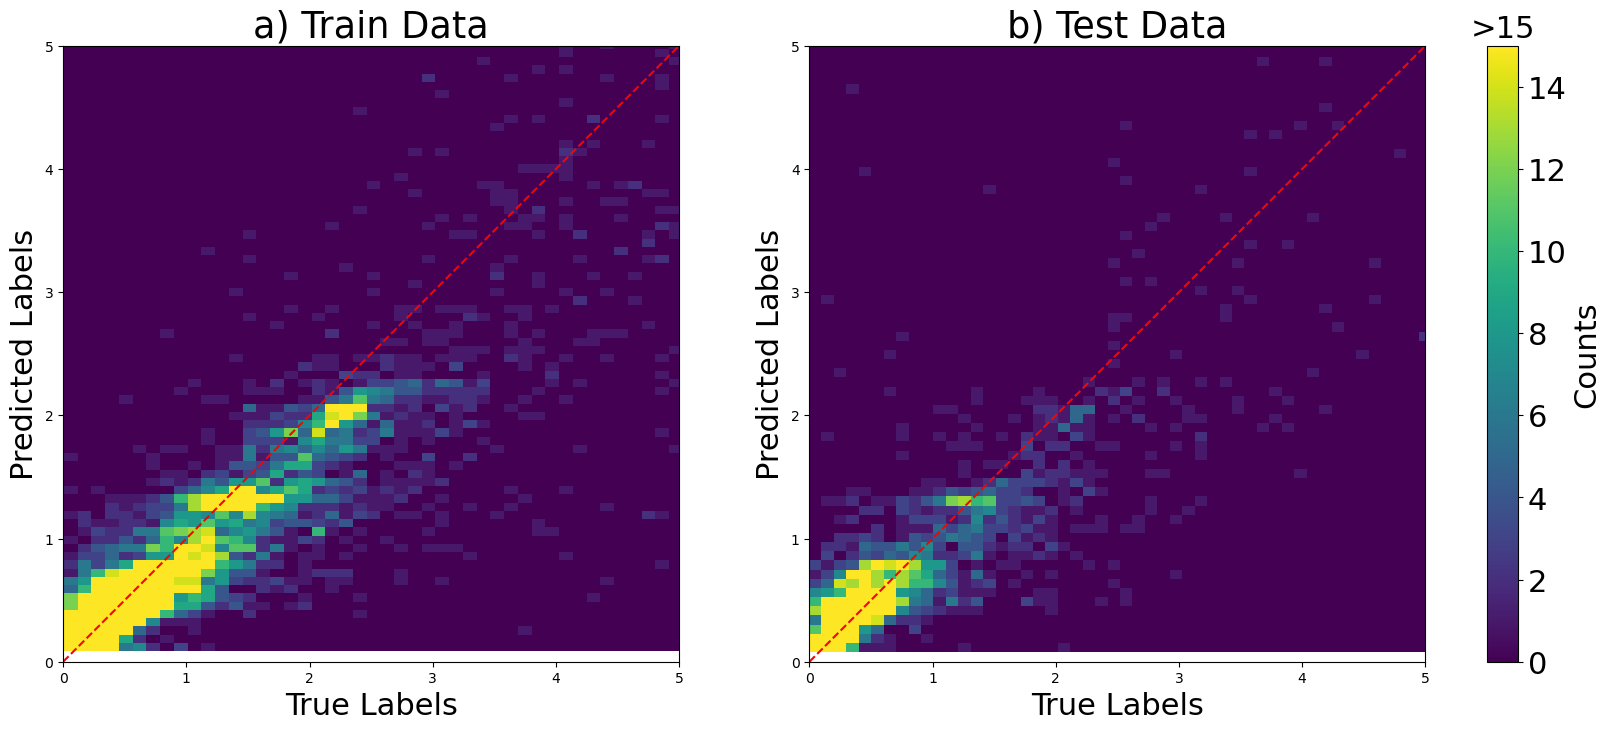
\includegraphics[width = 12 cm]{figures/f02.png}
    \caption{Heat map of the correlation plot between measured (labels) and predicted data (targets) using DNN for a) train data and b) test data, to assess the model performance. The minimal difference observed between train and test errors serves as an indicator of the model's ability to avoid overfitting.}
    \label{fig:correlationPlot}
\end{figure}



\begin{figure}
        \centering
        \includegraphics[width = 12cm]{figures/f03v2.png}
        \caption{Global prediction map of the TOC concentration using a DNN. Higher TOC concentration is observed in Arctic region and in upwelling areas located along the western continental margins of America and Africa, the equatorial Pacific, and the Arabian Sea.}
        \label{fig:tocPercent}
\end{figure}



Our DNN-based map of TOC concentrations (Figure \ref{fig:tocPercent}) shows similarities to maps previously published by \cite{SEITER20042001} and \cite{LeeTOCkNN}, who used geostatistical methods and a kNN model, respectively. All maps show elevated concentrations in the Arctic region and in upwelling areas located along the western continental margins of America and Africa, the equatorial Pacific, and the Arabian Sea. This pattern can be explained by elevated rates of marine primary and export production in upwelling regions delivering large fluxes of TOC to the seabed. The low TOC values in the open oceans are related to lower productivity and the large water depths limiting the TOC flux to the deep-sea floor. The predictions in Figure \ref{fig:tocPercent} are also consistent with the early work on TOC distributions by \cite{Berner1982} and \cite{Emerson1988}, showing low TOC values in the open oceans and elevated values for upwelling regions and the Arctic region. The high TOC concentrations predicted for the Black Sea and Baltic Sea (Figure \ref{fig:tocPercent}) are probably related to the lack of oxygen in bottom waters of these marginal seas that promotes TOC preservation \citep{HEDGES199581}. The map published by \cite{LeeTOCkNN} shows several large areas in the open Pacific that have unusually high TOC concentrations.  These patches are probably not realistic since they do not appear in other maps and are not consistent with our understanding of the TOC cycle. They may be artifacts generated by the kNN method and the sparse data coverage in these regions. Our new map avoids these artifacts and presents a pattern that better corresponds to our understanding of TOC accumulation in the seafloor for both the deep-sea and the continental shelf that were never modeled individually in previous maps.  


\begin{figure}
        \centering
	        \includegraphics[width = 12cm]{figures/f04v2.png}
        \caption{TOC stock map using the global porosity grid provided by \cite{Martin2005Porosity}. The color map is shown on a logarithmic scale.}
        \label{fig:tocStock}
\end{figure}

We also produced a map of TOC stocks for the global ocean (Figure \ref{fig:tocStock}). The TOC stock was calculated using the global porosity grid provided by \cite{Martin2005Porosity} and a density of dry solids ($d_s$) of $2.6 g/cm^3$. We performed the calculation for the top 10 $cm$ of the sediment column since our TOC data have been measured within this mixed surface layer. Moreover, the top 10 $cm$ are the most vulnerable and dynamic part of the sedimentary TOC pool since they are subject to frequent biological and physical mixing  processes \citep{song2022global} and are affected by human interventions such as bottom trawling \citep{Sala2021}.

\begin{equation}
 \text{TOC stock} = (1 - \text{porosity}) \times d_s \times \text{TOC concentration} \times \text{10 cm}   
 \label{eq:stock}
\end{equation}


\begin{table}[htbp]

\centering
\begin{tabular}{|p{0.2\textwidth}|p{0.1\textwidth}|p{0.1\textwidth}|p{0.1\textwidth}||p{0.1\textwidth}|p{0.1\textwidth}|p{0.1\textwidth}|}
\hline
& \multicolumn{3}{c||}{\textbf{Continental shelves}} & \multicolumn{3}{c|}{\textbf{Deep-sea}} \\
\hline
\textbf{Region} & \textbf{Sum of TOC stock ($Pg$)} & \textbf{Area (million km\textsuperscript{2})} & \textbf{Mean TOC concentration (\%)} & \textbf{Sum of TOC stock ($Pg$)} & \textbf{Area (million km\textsuperscript{2})} & \textbf{Mean TOC concentration (\%)} \\
\hline
\hline
Arctic Ocean & 5.57& 5.72 & 0.94& 7.18& 9.46 & 0.88\\
\hline
Indian Ocean & 2.63& 4.06 & 0.61& 25.86& 67.10 & 0.55\\
\hline
Mediterranean Region & 0.61& 0.65 & 0.98& 1.95& 2.27 & 1.04\\
\hline
North Atlantic Ocean & 2.82& 4.26 & 0.63& 14.96& 37.46 & 0.58\\
\hline
North Pacific Ocean & 2.74& 3.83 & 0.66& 31.16& 73.42 & 0.67\\
\hline
South Atlantic Ocean & 1.25& 1.86 & 0.82& 12.76& 38.67 & 0.51\\
\hline
South China and Easter Archipelagic Seas & 1.56& 3.00 & 0.48& 2.58& 3.74 & 0.83\\
\hline
South Pacific Ocean & 1.26& 1.46 & 1.02& 32.96& 83.81 & 0.58\\
\hline
Southern Ocean & 0.21& 0.57 & 0.59& 6.39& 20.16 & 0.43\\
\hline
Baltic Sea$^*$ & 0.77& 0.39 & 3.03& & & \\
\hline
Caspian Sea$^*$ & 0.72& 0.38 & 2.27& & & \\
\hline
\hline
\textbf{Total} & 20.15& 26.20 & 0.79& 135.80& 336.08 & 0.59\\
\hline
\end{tabular}
\caption{TOC Stock in the continental shelf  and deep-sea regions. $^*$The total sums and the mean concentrations in the continental shelves include the Baltic Sea and the Caspian Sea. Without these regions, the total TOC stock in continental shelves is 18.66 $Pg$, area of the continental shelves is 25.42 million km\textsuperscript{2} and the mean TOC concentration is 0.66\%. }
\label{tab:TOCStockOcean} 
\end{table}









The TOC stock is computed for global oceans and major seas \citep{FlandersMarineInstitute2021},  considering both continental shelves and deep-sea regions within each ocean and sea (Table \ref{tab:TOCStockOcean}. Notably, the mean TOC concentration in continental shelves exhibits significant variability across regions. Visualization of the TOC stock in the oceans is provided in Appendix \ref{appendix:tocStockDiffMarine}.

According to our  model, most the TOC stock can be found in the vast deep-sea basins of the Pacific, Indian and Atlantic oceans which is due to the large area of these basins (Table \ref{tab:TOCStockOcean}). The shelf region harbors 12.1\% of the global stock (Table \ref{tab:TOCStockOcean}, excluding Baltic Sea and Caspian Sea), similar to the fraction, previously derived by \cite{atwood2020} who suggested that 11.5\% of the global TOC stock is located on the continental shelves. The global TOC stock derived from our model amounts to 155.8 $Pg$ carbon for the 10 $cm$ layer consider in our calculations (Table \ref{tab:TOCStockOcean}). This value is close to the global stock in the top 10 $cm$ derived by reactive transport modeling (170 $Pg$, \cite{larowe2020b}). The other stock estimates were calculated applying a range of sediment thicknesses. When normalized to 10 $cm$, the stocks reported by \cite{LeeTOCkNN} amounts to 174 $Pg$ while the stock derived by \cite{atwood2020} results as 232 $Pg$ carbon. The first stock estimate, that was based on expert knowledge and a limited data base, corresponds to only 49 $Pg$ carbon when normalized to 10 $cm$ \citep{Emerson1988} which is lower than our estimate. Our new global stock assessment, hence, falls into the range of previous estimates.% in the low reactivity scenario 

According to our DNN-model, the mean TOC concentration in continental shelf sediments, excluding the Baltic Sea and the Caspian Sea (0.70\%) is close to the concentration in deep-sea sediments (0.59\%, Table \ref{tab:TOCStockOcean}). This is a surprising result since the high marine productivity and low water depths on the shelf induce high TOC fluxes to the seabed that should result in elevated TOC concentrations in surface sediments. Moreover, large amounts of terrestrial particulate organic carbon (POC) produced by land plants are deposited in shelf sediments \citep{Burdige2005} which should further increase TOC concentrations in these deposits. However, TOC concentrations in shelf surface sediments are diminished by a number of factors: i.  frequent biological and physical reworking that accelerates TOC degradation processes \citep{song2022global}, ii. dilution of TOC by inorganic material (clay, silt, sand) in delta deposits and other shelf regions with high sedimentation rates \citep{Berner1982}, iii. strong bottom currents that inhibit sediment deposition such that large shelf areas are covered by relict coarse-grained sediments that were deposited in the geological past and do not contain significant amount of TOC \citep{emery1968relict}, iv: frequent bottom trawling that exposes sedimentary TOC to oxygen and accelerates TOC degradation \citep{atwood2020}. According to our DNN-model, these factors could potentially decrease TOC concentrations in shelf sediments to such to degree that they attain mean values that are close to those observed in deep-sea sediments (Table \ref{tab:TOCStockOcean}). It should, however, be noted that most TOC burial occurs on the shelf where sedimentation rates are elevated due to the deposition of riverine particles \citep{Bradley2022}.

A method based on cooperative game theory (SHAP , SHapley Additive exPlanations), is used to further analyze our results and identify features that have a large effect on the predicted distribution of TOC concentrations \citep{lundberg2017shap}. The higher the SHAP value for a feature, the more important is the feature for the predictions of that particular model According to our model analysis, the total oxygen uptake feature \citep{TOU_JORGENSEN2022} has the largest effect (SHAP value) on predicted TOC concentrations in shelf sediments while the global porosity grid \citep{Martin2005Porosity} was the most important feature for deep-sea sediments It should, however, be noted that the feature importance ranking is only valid for our specific model set-up and might not be representative for the real world. Model interpretability and feature importance ranking is further discussed in Appendix \ref{appendix:shap}.

To guide future sampling, a new information gain map is provided (Figure \ref{fig:informationgain}). It identifies the regions that should be explored to improve the current model predictions. Some of the main takeaways from the information gain map are: i. Regions with high information gain are found in parts of the equatorial Pacific Ocean, Zealandia and around Papa New Guinea. These regions are less explored geographically and hence the model is not trained with the features in this region. ii. The continental slopes at the western coast of North America, east of Iceland and parts of the eastern coast of Africa have higher information gain, though they have more measurements. This could be due to the steep slopes and rough topography in these regions that may induce a high spatial heterogeneity in TOC values that is not yet resolved by the model. iii. Though the Southern Ocean is not well explored, the higher information gain regions are only found in regions with relatively steep terrain such as areas located close to islands and ocean ridges. These examples show that an abundance of measurements does not necessarily correspond to lower information gain, and vice versa. Information gain depends not only on the geographical proximity of measurements but also on their proximity in the parameter space and the congruence of the measurements made there. Including measurements from a region of higher information gain should lead to higher model knowledge and hence are more valuable compared to regions of low information gain. An experiment showing this is presented in Appendix \ref{appendix:informationgain}.


\begin{figure}
    \centering
    \includegraphics[width = 12cm]{figures/f05v2.png}
    \caption{The information gain map serves as a guide for determining optimal sampling locations, i.e. those with high information gain values. The color scheme highlights the high information gain regions with brighter colors. Information gain does not have any units, and is non-negative, $[0, inf)$.}
    \label{fig:informationgain}
\end{figure}



\section{Conclusions}  %% \conclusions[modified heading if necessary]
The comparison between different modeling approaches, including DNNs, kNNs, and random forests, highlights the effectiveness of each method in predicting TOC concentrations. While kNN and random forest models exhibit higher correlation coefficients and overall performance on the training dataset, the DNN outperforms them on test data performance. This suggests a potential overfitting issue with the kNN and random forest models, where they may have become specialized in learning the training data. Nonetheless, these algorithms remain useful, especially when computational resources are limited.

Our DNN-based map of TOC concentrations shows elevated concentrations in specific regions such as the Arctic and upwelling areas along continental margins. These patterns are consistent with known processes of marine primary and export production. Notably, our model that treats the shelf and deep-sea regions as separate entities captures their individual dynamics with higher accuracy and yields a better global map of TOC concentrations than a model version that simulates the entire ocean as one continuous system. It specifically avoids  artifacts like unrealistic high TOC concentrations in  open ocean regions with poor data coverage that have also been encountered in previous kNN and forest models.

The computed TOC stock for global oceans and major seas provides valuable insights into the distribution and magnitude of TOC storage. Despite significant variability in mean TOC concentration across continental shelves, our model confirms that the majority of the TOC stock is found in deep-sea basins. Surprisingly, mean TOC concentrations in continental shelves are close to those in deep-sea sediments, suggesting complex processes at play that diminish TOC concentrations in shelf sediments.

The analysis of information gain highlights regions with sparse or contradicting measurements and higher uncertainty, providing guidance for future sampling efforts. It reveals that the abundance of measurements does not necessarily correspond to lower uncertainty, emphasizing the importance of considering both geographical proximity and parameter space proximity in sampling strategies.

In conclusion, our study contributes to a better understanding of global TOC distributions and stocks, shedding light on the complex interplay between biological, physical, and geological processes in marine sedimentary environments. The insights gained from our modeling approach can inform future research and management efforts aimed at preserving and managing marine carbon sinks.


\codeavailability{The repository of code to run the different models, analyse the outputs is available at: \url{https://doi.org/10.3289/SW_3_2024}.} 

\dataavailability{Raw features and labels, model outputs are available at: \url{https://doi.org/10.5281/zenodo.11186224}.} 


\appendix

\makeatletter
\def\@seccntformat#1{\@ifundefined{#1@cntformat}%
   {\csname the#1\endcsname\space}%    default
   {\csname #1@cntformat\endcsname}}%  enable individual control
\newcommand\section@cntformat{\appendixname\thesection.\space} % section-level
\makeatother
\renewcommand{\thesection}{S\arabic{section}}
\counterwithin{equation}{section}
\counterwithin{figure}{section}
\counterwithin{table}{section}

%\section*{Appendices}
%\addcontentsline{toc}{section}{Appendices}
%\renewcommand{\thesection}{\Alph{section}}
\section{Feature list}
\label{appendix:featurelist}

File names adhere to the naming conventions discussed below. The naming structure is partitioned by underscores and periods in the following order: interface to which the gridded values refer to, quantity of values contained within the grid, units and reference values/units (e.g. meters below sea level), data source, statistic calculated (if applicable), grid pitch, and file extension.


SS – Sea surface – atmosphere interface (may also be average of the entire water column);

SF – Seafloor – water interface (may also be denoted by GL- Ground level);

 (r50 km) - Raw feature and feature averaged at a 50km radius used.

Units referenced are as follows:

KGM3 - kilogram per cubic meter;

MS - meters per second;

KM - kilometer;

M\_ASL - meters above sea level (i.e. meters referenced to sea level);

MWM2 - milliwatt per square meter;

TGCYR - terragram of carbon per year;

TGYR - terragram per year;

MA - megaannum;

M - meters;

MGCM2 - milligram of carbon per square meter;

DEG - degree;

S - seconds.

Most of the features presented below have been collected by  \cite{lee_2020_3675364} and \cite{benjamin_j_phrampus_2019_3459805}. The new datasets including the additions from this work are uploaded at \url{https://doi.org/10.5281/zenodo.11186224}.


\begin{longtable}{|p{0.4\textwidth}|p{0.35\textwidth}|p{0.25\textwidth}|}
    \hline
      \textbf{Feature} & \textbf{Explanation} & \textbf{Data Source} \\
      \hline
      \endfirsthead
      \hline
      \textbf{Feature name} & \textbf{Explanation} & \textbf{Data Source} \\
      \hline
      \endhead
        GL \_COAST \_FROM \_LAND \_IS \_1.0 \_ETOPO2v2.5m.nc (raw, r50km) & Coastline, with a binary indicator for the presence of coastline. This dataset is derived from ETOPO2v2, a 2-minute gridded global relief data for land topography  &  \cite{ETOPO2v22006}\\
        \hline 
        GL \_COAST \_FROM \_SEA \_IS \_1.0 \_ETOPO2v2.r50km.men.5m.nc (raw, r50km) & Coastline with a binary indicator for the presence of coastline using ETOPO2v2 relief data for ocean bathymetry & \cite{ETOPO2v22006} \\
        \hline 
        GL \_DIST \_TO \_COAST \_KM \_ETOPO.r50km.men.5m.grd (raw, r50km)&  Distance of ocean grid points to the nearest coast. & \cite{ETOPO2v22006} \\
        \hline 
        GL \_ELEVATION \_M \_ASL \_ETOPO2v2.r50km.men.5m.grd (raw, r50km)&  Elevation data from ETOPO2v2, representing heights above sea level & \cite{ETOPO2v22006} \\
        \hline 
        GL \_RIVERMOUTH \_CO2 \_TGCYR-1 \_ORNL.r50km.men.5m.grd (raw, r50km)& Carbon dioxide flux at river mouths, measured in teragrams of carbon per year (Tg C/yr) &  \cite{ONRL2011}\\
        \hline 
        GL \_RIVERMOUTH \_DOC \_TGCYR-1 \_ORNL.r50km.men.5m.grd (raw, r50km)& Dissolved organic carbon flux at river mouths (Tg C/yr) & \cite{ONRL2011} \\
        \hline 
        GL \_RIVERMOUTH \_HCO3 \_TGCYR-1 \_ORNL.r50km.men.5m.grd (raw, r50km)& Bicarbonate \ce{HCO3-} flux at river mouths (Tg C/yr) & \cite{ONRL2011} \\
        \hline 
        GL \_RIVERMOUTH \_POC \_TGCYR-1 \_ORNL.r50km.men.5m.grd (raw, r50km)& Particulate organic carbon flux at river mouths (Tg C/yr) &  \cite{ONRL2011}\\
        \hline 
        GL \_RIVERMOUTH \_TSS \_TGYR-1 \_ORNL.r50km.men.5m.grd (raw, r50km) & Total suspended solids flux at river mouths (50 km resolution) (Tg C/yr). All riverine fluxes are binary features with the magnitude of fluxes defined at the coastline and a value of zero for the ocean's interior & \cite{ONRL2011} \\
        \hline 
        %\newpage
        GL \_TOT \_SED \_THICK \_M \_CRUST1 \_NOAA.r50km.men.5m.grd (raw, r50km) & Total sediment thickness in the earth's crust in $m$  & \cite{CRUST1_NOAA2013} \\
        \hline 2N2 \_ocean \_eot20 \_modified.nc;K1 \_ocean \_eot20 \_modified.nc;K2 \_load \_eot20 \_modified.nc;K2 \_ocean \_eot20 \_modified.nc;M2 \_load \_eot20 \_modified.nc;M2 \_ocean \_eot20 \_modified.nc;M4 \_load \_eot20 \_modified.nc;M4 \_ocean \_eot20 \_modified.nc;MF \_load \_eot20 \_modified.nc;MF \_ocean \_eot20 \_modified.nc;MM \_load \_eot20 \_modified.nc;MM \_ocean \_eot20 \_modified.nc;N2 \_load \_eot20 \_modified.nc;N2 \_ocean \_eot20 \_modified.nc;O1 \_load \_eot20 \_modified.nc;O1 \_ocean \_eot20 \_modified.nc;P1 \_load \_eot20 \_modified.nc;P1 \_ocean \_eot20 \_modified.nc;Q1 \_load \_eot20 \_modified.nc;S1 \_load \_eot20 \_modified.nc;S1 \_ocean \_eot20 \_modified.nc;S2 \_load \_eot20 \_modified.nc;S2 \_ocean \_eot20 \_modified.nc;SA \_load \_eot20 \_modified.nc;SA \_ocean \_eot20 \_modified.nc; SSA\_load\_eot20\_modified.nc; SSA\_ocean\_eot20\_modified.nc & \cite{HartDavis2021EOT20} provides global atlases of both ocean and load tides, containing information about the amplitudes and phases of seventeen tidal constituents (ocean and load) for the global ocean. These constituents include: 2N2, J1, K1, K2, M2, M4, MF, MM, N2, O1, P1, Q1, S1, S2, SA, SSA, and T2, that extends across the entire global ocean ranging from 66°S to 66°N. For higher latitudes, the FES2014b model is used to fill in the gaps. Eleven satellite altimetry missions contribute to this model. & \cite{HartDavis2021EOT20} \\
        \hline 
        ChlorSummerMean.nc & Average chlorophyll-a concentration during summer (June to November), collected from July 2002 till July 2022 &  \cite{nasaaqua}\\
        \hline 
        ChlorWinterMean.nc & Average chlorophyll-a concentration during winter (Decmeber to May), collected from July 2002 till July 2022 &  \cite{nasaaqua}\\
        \hline 
        DERIVATIVE \_GL \_ELEVATION \_M \_ASL \_ETOPO2v2.5.nc & Slope from ETOPO2v2.5 data &  \\
        \hline 
        GL \_HEATFLUX \_MWM2 \_Becker.5m.nc & Oceanic heat flux data (exchange of heat energy between the ocean surface and the atmosphere) in megawatts per square meter ($MW/m^2$) & \cite{becker2014} \\
        \hline
        GL \_LAND \_IS \_1.0 \_ETOPO2v2.5m.nc & Land mask data & \cite{ETOPO2v22006} \\
        \hline 
        POROSITY \_global \_prediction.grd & Global prediction map for porosity of surface sediments using a random forest method  & \cite{Martin2005Porosity} \\
        \hline 
        SF \_ACTIVE \_SEAMOUNTS \_KIM.r10km.wct.5m.grd & Active (volcanically) seamounts location data at a 10 km resolution & \cite{KIM2011} \\
        \hline 
        SF \_AVG \_SEA \_DENSITY \_KGM3 \_DECADAL \_MEAN \_woa13x.5m.grd (raw, r50km)& Sea density in $kg/m^3$, averaged   &  \cite{WOA13X2013}\\
        \hline 
        SF \_COASTLINE \_IS \_1.0.5m.nc & Coastline data from Global Land One-kilometer Base Elevation (GLOBE) &  \cite{ETOPO2v22006}\\
        \hline 
2        SF \_CURRENT \_EAST \_MS \_2012 \_12 \_HYCOMx.5m.grd;SF \_CURRENT \_NORTH \_MS \_2012 \_12 \_HYCOMx.5m.grd;SF \_CURRENT \_MAG \_MS \_2012 \_12 \_HYCOMx.5m.grd (raw, r50km)& Ocean bottom current data for the east-west, north-south component and total magnitude using the HYCOM model in $m/s$.  The data is provided in 1/12 $\°$ resolution. The dataset has a time range from August 1, 1995 to December 31, 2012, temporally averaged.  & \cite{HYCOM2014} \\
        \hline  
        SF \_GRAINSIZE \_D16 \_MM \_NGDC.5m.nc;SF \_GRAINSIZE \_D50 \_MM \_NGDC.5m.nc;SF \_GRAINSIZE \_D84 \_MM \_NGDC.5m.nc & Grainsize data with the 16th percentile (D16), median (D50) and the 84th percentile (D84) & \cite{ngdc1976} \\
        \hline 
        SF \_SEA \_BULKMODULUS \_MPA \_DECADAL \_MEAN \_woa13x.5m.nc & Sea bulk modulus in mega pascals (MPa) averaged over six decades, from the year 1955 to 2012. The sea bulk modulus is an important thermodynamic property and is a measure of resistance against the compressibility of a fluid. It is calculated from  the  International Equation of State of Seawater from \cite{UNESCO1991}  & \cite{WOA13X2013} \\
        \hline 
        SF \_SEA \_CONDUCTIVITY \_SM \_DECADAL \_MEAN \_woa13v2x.5m.grd (raw, r50km)  & Average conductivity of seawater (dissolved ions) at the sea surface over six decades, from the year 1955 to 2012 and the units are in Siemens per meter ($S/m$) & \cite{WOA13X2013} \\
        \hline 
        SF \_SEA \_OXYGEN \_MLL \_DECADAL \_MEAN \_woa13v2x.5m.grd (raw, r50km) & Average dissolved oxygen concentration in seawater in millilitre per litre over a decadal mean & \cite{WOA13X2013} \\
        \hline 

        SF \_SEA \_OXYGEN \_PCTSAT \_DECADAL \_MEAN \_woa13v2x.5m.grd (raw, r50km) & Oxygen concentration in seawater percentage saturation averaged over six decades, from the year 1955 to 2012. & \cite{WOA13X2013}\\
        \hline 
        SF \_SEA \_PRESSURE \_MPA \_DECADAL \_MEAN \_woa13x.5m.nc & Seawater pressure in mega pascals ($MPa$) averaged over six decades, from the year 1955 to 2012. & \cite{WOA13X2013} \\
        \hline 
        SF \_SEA \_SALINITY \_PSU \_DECADAL \_MEAN \_woa13v2x.5m.nc & Seawater salinity in practical salinity units averaged over six decades, from the year 1955 to 2012. & \cite{WOA13X2013} \\
        \hline 
        SF \_SEA \_SEA \_OXYGEN \_UTILIZATION \_MOLM3 \_DECADAL \_MEAN \_woa13v2x.5m.grd (raw, r50km) & Oxygen concentration in seawater utilization in mol/m³ averaged over six decades, from the year 1955 to 2012. &  \cite{WOA13X2013}\\
        \hline 
        SF \_SEA \_TEMPERATURE \_C \_DECADAL \_MEAN \_woa13v2x.5m.grd (raw, r50km) &  Seawater Temperature in Celcius averaged over six decades, from the year 1955 to 2012. & \cite{WOA13X2013} \\
        \hline 
        SL \_GEOID \_M \_ABOVE \_WGS84 \_NGA \_egm2008.5m.grd & Height of the geoid above the WGS84 reference ellipsoid, in meters ($m$), and referenced to the National Geospatial-Intelligence Agency (NGA)
& \cite{NGA_EGM20082008} \\
        \hline 
        SS \_BIOMASS \_BACTERIA \_LOG10 \_MGCM2 \_WEI2010x.5m.grd (raw, r50km); SS \_BIOMASS \_FISH \_LOG10 \_MGCM2 \_WEI2010x.5m.grd (raw, r50km); SS \_BIOMASS \_INVERTEBRATE \_LOG10 \_MGCM2 \_WEI2010x.5m.grd (raw, r50km); SS \_BIOMASS \_MACROFAUNA \_LOG10 \_MGCM2 \_WEI2010x.5m.grd (raw, r50km); SS \_BIOMASS \_MEGAFAUNA \_LOG10 \_MGCM2 \_WEI2010x.5m.grd (raw, r50km); SS \_BIOMASS \_MEIOFAUNA \_LOG10 \_MGCM2 \_WEI2010x.5m.grd (raw, r50km); SS \_BIOMASS \_TOTAL \_LOG10 \_MGCM2 \_WEI2010x.5m.grd (raw, r50km); & Distribution of mean biomass predictions for (a) bacteria, (b) fishes, (c) invertebrates, (d) macrofauna, (e) megafauna, and (f) meiofauna. The mean biomass was computed using random forest algorithm. The total biomass was combined from predictions of bacteria, meiofauna, macrofauna, and megafauna biomass. Predictions were smoothed by Inverse Distance Weighting interpolation to 0.1 degree resolution and displayed in logarithm scale (base of 10), which is then converted to 5 arc minute grids by \cite{LeeTOCkNN} & \cite{WEI2010} \\
        \hline 
        SS \_CHLOROPHYLL \_LOG \_MG \_M3 \_MODIS \_Aqua \_MISSION \_MEANx.5m.grd (raw, r50km); SS \_PIC \_LOG \_MOL \_M3-1 \_MODIS \_Aqua \_MISSION \_MEANx.5m.grd (raw, r50km); SS \_POC \_LOG \_MOL \_M3-1 \_MODIS \_Aqua \_MISSION \_MEANx.5m.grd (raw, r50km)  & The Moderate Resolution Imaging Spectroradiometer (MODIS), is a 36-band spectroradiometer measuring visible and infrared radiation and obtaining data that are being used to derive the near-surface concentration of chlorophyll-a (chlor\_a) in $mg m^-3$. It is calculated using an empirical relationship derived from in situ measurements of chlor\_a, concentrations of Particulate Organic Carbon (POC) and Particulate Inorganic Carbon (PIC) (i.e., calcium carbonate or calcite) and blue-to-green band ratios of in situ remote sensing reflectances (Rrs). & \cite{nasaaqua} \\
        \hline 
        SS \_CORIOLIS.5m.nc  & Coriolis data, generated using empirical means & \cite{lee_2020_3675364}\\
        \hline 
        SS \_DENSITY \_KGM-3 \_SACD \_Aquarius \_MISSION \_MEANx.5m.grd & The Aquarius/SAC-D satellite mission, launched on 10 June 2011, was a joint venture between NASA and the Argentinean Space Agency (CONAE). The mission featured the sea surface salinity sensor Aquarius and was the first mission with the primary goal of measuring sea surface salinity (SSS) from space. The monthly maps of sea surface density are derived from Aquarius sea surface salinity and ancillary sea surface temperature. The time period used to average is between 25 August 2011 to 07 June 2015.  & \cite{nasaaquarius} \\
        \hline 

         SS \_GEOID \_ANOMALY \_NGA \_egm2008.5m.nc (raw, r50km) & The regional Free-air and Bouguer gravity anomaly grids (averaged over 2,5 arc-minute by 2,5 arc-minute) are computed at BGI from the EGM2008 spherical harmonic coefficients & \cite{NGA_EGM20082008} \\
        \hline 
        SS \_MIXED \_LAYER \_DEPTH \_MAX \_M \_Goyetx.5m.grd (raw, r50km); 
         SS \_MIXED \_LAYER \_DEPTH \_MIN \_M \_Goyetx.5m.grd (raw, r50km)& Shows the geographical distribution of the maximum and minimum depth ($m$) of the mixed layer. The observations are in the time span between March 1995 and February 1996. & \cite{goyetMLD} \\
        \hline
        
        SS \_PHOTO \_AVAIL \_RAD \_EINSTEIN \_M-2 \_DAY \_SNPP \_VIIRS \_MISSION \_MEANx.5m.grd (raw, r50km); SS \_PHYTO \_ABSORPTION \_443NM \_M-1 \_SNPP \_VIIRS \_MISSION \_MEANx.5m.grd  & Daily average photosynthetically available radiation (PAR) at the ocean surface in $Einstein/m^2/day$ The Visible Infrared Imaging Radiometer Suite (VIIRS) on the Suomi National Polar-orbiting Partnership (SNPP) have been developed for global ocean color products. PAR is defined as the quantum energy flux from the Sun in the 400-700nm range. For ocean color applications, PAR is a common input used in modeling marine primary productivity. An average of the sensors and the 443 $nm$ wavelength maps are used as features& \cite{nasaaqua}\\
        \hline
        
        
         SS \_WAVE \_DIRECTION \_DEG \_2012 \_12 \_WAVEWATCH3x.5m.grd (raw, r50km); SS \_WAVE \_HEIGHT \_M \_2012 \_12 \_WAVEWATCH3x.5m.grd (raw, r50km); SS \_WAVE \_PERIOD \_S \_2012 \_12 \_WAVEWATCH3x.5m.grd (raw, r50km) & Mean Wave direction in $\°$, wave height in $m$ and wave period in $s$. The data is provided in 1/12 $\°$ resolution. The dataset is averaged over the time range from August 1, 1995 to December 31, 2012. Features are based on the 3rd generation wave model WAVEWATCH III®. & \cite{HYCOM2014} \\   
        \hline 
        
        
        SS \_WINDSPEED \_MS-1 \_SACD \_Aquarius \_MISSION \_MEANx.5m.grd (raw, r50km) & Mean wind speed in $m/s$ from the Aquarius/SAC-D satellite mission. The time period used to average is between 25 August 2011 to 07 Jun 2015.  & \cite{nasaaquarius} \\
        \hline 
        
        
        TOU \_Jorgenson2022.nc & Global map of the total oxygen uptake (TOU) of the seabed. & \cite{TOU_JORGENSEN2022} \\
        \hline 
  		\newpage      
        
        litho\_maps\_type1\_.nc & Lithology map: Mudflats binary map (Median grain size <0.05 $mm$) & \cite{garlan2018}  \\
        \hline 
        
        
        litho\_maps\_type2\_.nc & Lithology map: Fine sand binary map (Median grain size: 0.05 $mm$ - 0.5 $mm$) & \cite{garlan2018} \\
        \hline 
        
        
        litho\_maps\_type3\_.nc & Lithology map: Sand binary map (Median grain size: 0.5 $mm$ - 2 $mm$) & \cite{garlan2018} \\
        \hline 
        
        
        litho\_maps\_type4\_.nc & Lithology map: Clay binary map (Median grain size: <0.01 $mm$) & \cite{garlan2018}
        \hline 
        
        
        litho\_maps\_type5\_.nc & Lithology map: Gravel and stone binary map (Median grain size: >2 $mm$) & \cite{garlan2018}
        \hline 
        
        
        litho\_maps\_type6\_.nc & Lithology map: Bed rock binary map & \cite{garlan2018}
        \hline 
        
        
        lithology \_grain \_size \_global \_8.nc & Global seabed sediment map with 24 different classes or types of sediments based on a logarithmic progression of median grain size.  & \cite{garlan2018} \\
        \hline 
\caption{Feature list with description and references, that is used as input to all the models in the paper.}
\label{tab:myfirstlongtable}
\end{longtable}

\newpage
\section{Information gain}
\label{appendix:informationgain}
In this paper, KL divergence, also known as information gain or relative entropy, has been used to quantify model uncertainty. As \cite{renyi1961measures} points out, in the absence of observational information, the amount of information can be taken numerically equal to the amount of uncertainty concerning the model prediction. The mathematical derivation of KL divergence under the theoretical background of information theory \citep{shannoninformationgain1948} is presented below. The information entropy of a random variable $X$, with a probability distribution $P$ is represented as: 
\begin{equation}
\label{eq:entropy}
    H (P) = -\sum_i P (x_i) \log P (x_i)
\end{equation}

\cite{shannoninformationgain1948}'s definition of entropy determines the minimum channel capacity required to reliably transmit the information as encoded binary digits. Usually, the true distribution $P (X)$ denotes observed data, measurements, or an exact probability distribution. Here, $P (X)$ is constructed using a normal distribution with a mean value equal to Monte Carlo dropout prediction, and a standard deviation of 0.05 TOC\%, which arises from both technical handling and the precision of the weighing tool \citep{pape2020}. The predicted distribution $Q (X)$ is derived from the Monte Carlo dropout prediction ensemble. The measure $Q (X)$ typically represents a theoretical framework, a model, a description, or an approximation of $P (X)$. The cross entropy between $P (X)$ and $Q (X)$ measures the average number of binary digits to represent an event from $P (X)$, by $Q (X)$. It is represented as:

\begin{equation}
\label{eq:crossentropy}
    H (P, Q) = -\sum_i P (x_i) \log Q (x_i)
\end{equation}


The information gain measures the difference between the cross entropy (Equation \ref{eq:crossentropy}) and the entropy (Equation \ref{eq:entropy}), is represented as $D_{\text{KL}} (P \| Q)$. 

\begin{equation}
    D_{\text{KL}} (P \| Q) = H (P, Q) - H (P) = \sum_i P (x_i) \log\left (\frac{P (x_i)}{Q (x_i)}\right)
\end{equation}


$D_{\text{KL}} (P \| Q)$ is always non negative, remains well-defined for continuous distributions. To obtain the continuous distribution for the predicted distribution $Q (X)$, the prediction ensemble is binned into histograms, to obtain an approximate probability density function (PDF). This PDF is then modeled using curve fitting techniques, typically fitted to a Gaussian distribution (Algorithm \ref{alg:informationgain}). $D_{\text{KL}} (P \| Q)$, is calculated globally for each prediction, and plotted in the information gain map. 

In supervised machine learning, a model's predictive performance is usually determined by withholding a test dataset during the training phase and comparing the final model outputs to these known values. Such a procedure is not possible when evaluating the performance of information gain: firstly, the concept of a ground-truth for the information gain values does not exist. Secondly, we aim to measure the effect that data point selection guided by information gain has on the model output, and not on the information gain itself. Thus, in order to explore the effect that information gain has on data sampling and model refinement, we devised the following experiment:
A DNN model with the same parameters as the original one was trained while withholding one-third of the original training dataset: $\phi_{wh} (x, W, b)$. Afterwards, this model was used to calculate the information gain for each point in the withheld data. These additional data points were sorted according to their information gain values and divided into two subsets of equal size. Each of these subsets was used along with the initial two-thirds to train two new DNN models: one with added high information gain data points ($\phi_{wh+high\_ig} (x, W, b)$), and one with added low information gain data points ($\phi_{wh+low\_ig} (x, W, b)$). To validate for the entirety of the training data, the process was repeated two more times, withholding a different third of the dataset each time. 

In two of the three executions, the (test) performance of $\phi_{wh+high\_ig} (x, W, b)$ was superior to that of $\phi_{wh+low\_ig} (x, W, b)$ (Table \ref{tab:infogainexperiment}).
While the difference in performance from the different data subset might be small in magnitude, the selection of high information gain points also has a positive effect in the structure of the global inference patterns: in figure \ref{fig:infogaindiff} we took the prediction maps for both models of the worst performing data subset, $\phi_{wh+high\_ig} (x, W, b)_2$ and $\phi_{wh+low\_ig} (x, W, b)_2$, and calculated the absolute difference between them and the inference map of the original model $\phi (x, W, b)$ in figure \ref{fig:tocPercent}. Regardless of the performance metrics, the high information gain model resembles the  output of the original model more closely than the low information one.


\begin{figure}[!htb]
    \centering
    \includegraphics[width = 12 cm]{figures/f12.png}
    \caption{Top left: Difference in the prediction of TOC concentration between $\phi (x, W, b)$ and $\phi_{wh+low\_ig} (x, W, b)_2$; Top right: Difference in the prediction of TOC concentration between $\phi (x, W, b)$ and $\phi_{wh+high\_ig} (x, W, b)_2$. Brighter colors (shades of yellow) show higher difference and darker colors (shades of blue) show lesser difference; Bottom left (red box) : Zoomed in version of the equatorial Pacific region in a) and c), Bottom right (green box): Zoomed in version of the Caspian and the black sea in b) and d).}
    \label{fig:infogaindiff}
\end{figure}

\begin{table}[h]
  \centering
  \begin{tabular}{|l|c|c|c|c|c|c|}
    \hline
    \textbf{DNN model with different training datasets
    } & \multicolumn{3}{c|}{\textbf{Train data}} & \multicolumn{3}{c|}{\textbf{Test data (15\% of all data)}}  \\
    \hline
           & \textbf{Pearson CC} & \textbf{R-squared} & \textbf{MSE} & \textbf{Pearson CC} & \textbf{R-squared} & \textbf{MSE} \\
    \hline
    \textbf{$\phi_{wh+low\_ig} (x, W, b)_1$} & 0.918 & \textbf{0.840} & \textbf{0.535} & 0.814 & 0.641 & 0.692 \\
    \hline
    \textbf{$\phi_{wh+high\_ig} (x, W, b)_1$} & 0.918 & 0.833 & 0.586 & \textbf{0.825} & \textbf{0.679} & \textbf{0.640} \\
    \hline
    \hline
    \textbf{$\phi_{wh+low\_ig} (x, W, b)_2$} & \textbf{0.927} & \textbf{0.856} & \textbf{0.405} & \textbf{0.887} & \textbf{0.784} & \textbf{0.525}\\
    \hline
    \textbf{$\phi_{wh+high\_ig} (x, W, b)_2$} & 0.924 & 0.843 & 0.470 & 0.877 & 0.761 & 0.593 \\
    \hline
    \hline
    \textbf{$\phi_{wh+low\_ig} (x, W, b)_3$} & \textbf{0.935} & \textbf{0.864} & \textbf{0.410} & 0.819 & 0.668 & 0.575 \\
    \hline
    \textbf{$\phi_{wh+high\_ig} (x, W, b)_3$} & 0.932 & 0.853 & 0.428 & \textbf{0.855} & \textbf{0.728} & \textbf{0.475} \\
    \hline

  \end{tabular}
  \caption{Performance metrics of models trained on different subsets of data based on information gain for different splits of data (seeds): Pearson correlation coefficient (Pearson CC), coefficient of determination (R-Squared), and mean squared error for predicted values vs observed labels for the training and testing data. The train:test data ratio is 85:15.}
  \label{tab:infogainexperiment}
\end{table}




\newpage
\section{Comparison of methods}
\label{appendix:kNNRF}
One of the drawbacks of using DNN is the number of hyperparameters that needs to be tuned. The number of layers and nodes in each layer were decided on a trial and error method starting with the simplest configuration of 3 layers of 8 neurons. The model complexity was increased till the validation and the training performance was comparable, thus avoiding overfitting, but still getting relatively good performance on the test dataset. The initial learning rate was chosen based on the model convergence. The DNN model had 10 layers of 128 nodes each with a learning rate of 0.01. The batch size, decided based on the amount of data, was set as 500, was also chosen based on model convergence. On the other hand, the parameters that were tuned in the random forest algorithm and kNNs were the number of trees in the forest (controlled by number of estimators in sklearn) and number of neighbours respectively. They are tuned using the performance metrics for 1- 50 neighbours for kNN. number of estimators = 10, 20, 30, .. 100, for random forests. 

Though it is difficult to tune the DNN model, Table \ref{tab:kNNRF} highlights superior performance on the training dataset for kNNs and random forests, while their test performance or generalisation capability lags behind that of DNNs. Figure \ref{fig:tocPercent_kNN} and \ref{fig:tocPercent_RF}, the global predictions from kNNs and random forests respectively, show artifacts particularly in the equatorial Pacific and Atlantic oceans. 

%\appendixfigures  
\begin{figure}[!htb]
    \centering
    \includegraphics[width = 12 cm]{figures/f06v2.png}
    \caption{Global prediction map of TOC concentrations using a K-Nearest Neigbours algorithm with 5 nearest neighbors in the continental shelves and 4 nearest neighbors in the deep-sea. Spurious patches are observed in the equatorial Pacific ocean and in the Atlantic ocean.}%The total TOC stock from the random forests model is 164.27 $Pg$ and the mean TOC concentration is 0.63\% for the entire ocean.}
    \label{fig:tocPercent_kNN}
\end{figure}

\begin{figure}[!htb]
    \centering
    \includegraphics[width = 12 cm]{figures/f07v2.png}
    \caption{Global prediction map of TOC concentrations using a random forest algorithm with 100 estimators. Spurious patches are observed in the Atlantic ocean and the Bay of Bengal}% The total TOC stock from the random forests model is 155.14 $Pg$ and the mean TOC concentration is 0.60\% for the entire ocean.}
    \label{fig:tocPercent_RF}
\end{figure}



\newpage
\section{TOC stock in different marine regions}
\label{appendix:tocStockDiffMarine}
The table in Table \ref{tab:TOCStockOcean} breaks down how much TOC stock is found in different parts of the ocean. Each region is listed, showing how much TOC is there. Here we show a visualization of the different regions in Figure \ref{fig:TOCStockOceans}.

In Figure \ref{fig:TOCStockOceansWaffle}, we use a waffle chart to make it easier to see how the TOC is split among these regions. It's like dividing a pie into slices, but here we use squares. With a total of about 156 $Pg$ of TOC worldwide, the South Pacific Ocean gets the biggest share, while the Baltic Sea gets the smallest.
\begin{figure}[!htb]   
\centering
   \includegraphics[width = 12cm]{figures/f10.png}
   \caption{TOC stocks in different oceans}
   \label{fig:TOCStockOceans}
\end{figure}

\begin{figure}[!htb]
   \centering
   \includegraphics[width = 12cm]{figures/f11.png}
   \caption{TOC stocks in different oceans: Waffle chart}
   \label{fig:TOCStockOceansWaffle}
\end{figure}

\newpage
\section{DNN model run without separation of deep-sea and shelf environments}
\label{appendix:entireModel}
Here, we test a DNN model where the global ocean was not separated into shelf and deep-ocean regions but treated as one entity. The resulting TOC map shows spurious features in the Pacific Ocean , similar to those that occur in the map published by \cite{LeeTOCkNN}. These results underscore the importance of separating shelf and deep-ocean regions to achieve more accurate and realistic model outcomes.

\begin{figure}[!htb]
   \centering
   \includegraphics[width = 12cm]{figures/f13.png}
   \caption{TOC concentration map when the DNN model was not separated into shelf and deep-ocean regions. We see unrealistic TOC concentrations especially in the Pacific Ocean.}
   \label{fig:TOCConcEntireModel}
\end{figure}



\newpage
\section{Model interpretability using SHAP values}
\label{appendix:shap}
Explaining and understanding why a model makes a certain prediction is as crucial as accuracy and uncertainty in the predictions. This becomes particularly challenging in high-dimensional spaces, where interpreting complex models can be more intricate compared to simpler yet less accurate models. \cite{lundberg2017shap} propose SHAP (SHapley Additive exPlanations) as a unified framework for interpreting predictions. SHAP assigns importance values to each feature for a particular prediction, providing a comprehensive understanding of the model's decision-making process. In our supervised learning model $f$ trained on features $X \in \mathcal{X} \subseteq \mathbb{R}^d$ to predict outcomes $Y \in \mathcal{Y} \subseteq \mathbb{R}$, SHAP, a feature attribution method, considers the model predictions to be decomposed as a sum: $f (\mathbf{x}) = \phi_0 + \sum_{j=1}^{d} \phi (j, \mathbf{x})$, where $\phi_0$ is the baseline expectation (i.e., $\phi_0 = \mathbb{E}[f (\mathbf{x})]$) and $\phi (j, \mathbf{x})$ denotes the Shapley value of feature $j$ at point $x$. 


In our analysis, we aim to simplify the interpretation process by presenting the average importance of features across all predictions, from the deep-sea and the continental shelves. All effects describe the behavior of the model and are not necessarily causal in the real world. 

\begin{figure}[!htb]
\includegraphics[width=12cm]{figures/f08v2.png}
\caption{Summary plot of Shapley values of the deep-sea DNN model. The global porosity grid \citep{Martin2005Porosity} has the highest feature importance. Regions with high porosity lead to higher TOC concentrations, and vice versa. In the mechanistic model from \cite{Bradley2022}, porosity is positively correlated to the organic carbon flux through a specific depth. The biological features that includes total biomass, meiofauna and fish biomass in the sea surface \citep{WEI2010}, oxygen concentration in bottom waters \citep{WOA13X2013}, daily average PAR \citep{nasaaqua} show that higher biomass or marine productivity lead to higher TOC concentrations as expected. On the other hand, higher oxygen saturation leads to oxic conditions, resulting in the oxidation of the organic carbon and hence lower TOC concentration. The other features which dominate are the physical oceanographic features, where higher feature values result in lower TOC concentration, such as tidal features (Q1 loading) \citep{HartDavis2021EOT20}, sea bulk modulus \citep{WOA13X2013} and sea floor pressure \citep{WOA13X2013}.}
\label{fig:shap_do}
\end{figure}


\begin{figure}[!htb]
\includegraphics[width=12cm]{figures/f09v2.png}
\caption{Summary plot of Shapley values of the continental shelf DNN model. The total oxygen uptake \citep{TOU_JORGENSEN2022} of the seabed has the highest feature importance, with regions of higher oxygen uptake resulting in lower TOC concentrations, denoting oxic conditions. Regions with higher porosity \citep{Martin2005Porosity} result in higher TOC concentrations, while regions with lower porosity result in lower TOC concentration, but with lesser impact. The lithology map is a binary map. Regions with fine sand, with the grain size between 0.05 $mm$ and 0.5 $mm$ (1, being the higher feature value) have low TOC concentration. Higher sediment thickness in the earth’s crust lead to lower TOC concentration because of dilution \citep{Berner1982}. The bottom current components, north-south and east-west, result in reduced TOC concentration, due to higher resuspension of sediments, due to the inhibition of sedimentation, and hence burial of organic carbon. Higher average seawater conductivity results in lower TOC concentration. Higher Particulate Organic Carbon (POC) in the water column has a positive impact on the TOC concentrations, as expected. It can be seen that the feature importance is not as clearly defined as in the deep ocean (as the high (red) and the low (blue) feature values are mixed), because of the complex dynamics on continental shelves.}
\label{fig:shap_cs}
\end{figure}

\clearpage
The summary plot in Figures \ref{fig:shap_do} and \ref{fig:shap_cs} combines the feature importance with feature effects. The summary plot displays Shapley values representing the impact of features on predictions. Each point represents a Shapley value for a feature and an instance. The y-axis position indicates the feature, while the x-axis position corresponds to the Shapley value. Feature values are represented by color, ranging from low (blue) to high (red). To visualize feature importance, points are spread along the y-axis to reveal the distribution of Shapley values per feature. The features are ordered based on their importance, determined by the mean absolute Shapley values across all predictions. The Shapley value is expressed in the same units as the TOC concentration. This indicates the extent to which a specific feature value influences the TOC concentration, whether it drives it towards higher or lower values.










\newpage
\section{Algorithms}
\label{appendix:algorithms}
\begin{algorithm}
\caption{DNN Training with Batch Normalization and Dropout including Monte Carlo Dropout for inference}
\label{a2}
\begin{algorithmic}[1]
\REQUIRE Labeled dataset $D = \{ (x_1, y_1), (x_2, y_2), ..., (x_N, y_N)\}$ \\
\hspace{13mm} $x_i$: feature vector for the $i$th label \\
\hspace{13mm} $y_i$: corresponding TOC\%
\STATE \textbf{Input:} feature vector $x_j$
\STATE \textbf{Output:} Predicted TOC\% $\text{predicted\%}$ for $x_j$
\STATE \textbf{Method:} Construct a neural network with 10 layers and 128 nodes per layer: $\phi (x, W, b)$
\STATE Apply batch normalization and dropout to each layer.
\STATE Initialize optimizer (e.g., Adam) with appropriate learning rate and parameters.
\STATE Initialize loss function (e.g., Mean Squared Error) for regression.
\STATE Train the neural network with $D$ for 1000 epochs:
\FOR{$\text{epoch} = 1$ \TO $\text{num\_epochs}$}
    \STATE Randomly shuffle the training dataset..
    \FOR{$ (x_i, y_i)$ in $D$}
        \STATE Forward pass: compute predictions $\hat{y_i} = \phi (x_i, W, b)$.
        \STATE Compute target loss: $\text{loss}_{\text{target}} = \text{MSE} (y_i, \hat{y_i})$.
        \STATE Back-propagation: update weights and biases using optimizer, with $\text{loss}_{\text{target}}$ as the cost function.
    \ENDFOR
\ENDFOR
\STATE Set dropout to active during inference
\STATE Perform Monte Carlo dropout for $M$ forward runs:
\STATE \hspace{5mm} $\hat{y}^{\text{ensemble}}_j =  \phi (x_j, W, b, \text{dropout\_mask}_T)$
\STATE Predicted TOC\%, $\hat{y_j}$ for $x_j = \frac{1}{M}  \sum_{m=1}^{M} \hat{y}^{\text{ensemble}}_j$
\end{algorithmic}
\end{algorithm}

\begin{algorithm}
\caption{Calculating information gain for the predictions}
\label{alg:informationgain}
\begin{algorithmic}[1]
\REQUIRE Monte Carlo dropout prediction ensemble, $\hat{y}^{\text{ensemble}}$, for each grid cell
\FOR{each grid cell}
    \STATE Fit a gaussian probability density function $Q_j (x)$ for $\hat{y}^{\text{ensemble}}_j$ using histograms and curve fitting algorithm.
    \STATE Generate original distribution $P_j (x)$ with mean $\hat{y_j}$ and standard deviation 0.05 (sampling error).
    \STATE Calculate Kullback-Leibler divergence: \\
    \hspace{3mm} $D_{\text{KL}} (P_j \| Q_j) = \sum_i P_j (x_i) \log\left (\frac{P_j (x_i)}{Q_j (x_i)}\right)$
\ENDFOR
\end{algorithmic}
\end{algorithm}










\newpage
\authorcontribution{

Naveenkumar Parameswaran: data curation, formal analysis, investigation, methodology, software, validation, visualization, writing – original draft preparation

Everardo Gonz\'{a}lez: conceptualization, data curation, formal analysis, investigation, methodology, software, supervision, visualization, writing – original draft preparation

Ewa Burwicz-Galerne: data curation, investigation, methodology, supervision, validation, writing – original draft preparation

Malte Braack: funding acquisition, project administration, supervision, validation, writing – original draft preparation

Klaus Wallmann: conceptualization, funding acquisition, methodology, project administration, supervision, validation, writing – original draft preparation}

% \authorcontribution{Ewa Burwicz-Galerne conducted the data collection of the oceanographic features and TOC concentration labels. Klaus Wallmann and Ewa Burwicz-Galerne performed the feature selection and provided inputs on the geoscientific aspects of the manuscript. Malte Braack contributed to data cleaning and model building. Naveenkumar Parameswaran and Everardo Gonzalez conceptualized the idea and developed the model code and performed the runs. Naveenkumar Parameswaran prepared the manuscript with contributions from all co-authors.} 


\competinginterests{The authors declare that they have no conflict of interest.} %% this section is mandatory even if you declare that no competing interests are present

%\disclaimer{TEXT} %% optional section

\begin{acknowledgements}
This work was partially funded by the Cluster of Excellence `The Ocean Floor – Earth’s Uncharted Interface' (EXC 2077) financed by Deutsche Forschungsgemeinschaft (DFG) - Project number 390741603 hosted by the Research Faculty MARUM - Center for Marine Environmental Sciences, University of Bremen, Germany.

The first author wants to thank the Helmholtz School for Marine Data Science (MarDATA), for direct financial support.

The authors would like to thank Dr. Taylor R. Lee for her insightful review of the first submission of this work, which led to further improvement of the manuscript.

AI tools has been used to correct the manuscript, and optimize the code.
\end{acknowledgements}





\newpage
\bibliographystyle{copernicus}
\bibliography{ref.bib}


\end{document}
